\providecommand{\main}{..} 
\documentclass[\main/boa.tex]{subfiles}

\begin{document}

\section{Złożone schematy doboru próby - pakiet survey}
\begin{minipage}[t]{0.915\textwidth}
	\center     
    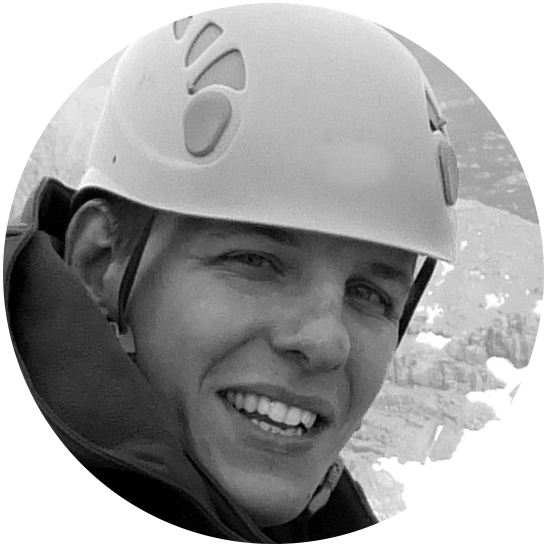
\includegraphics[width=60px]{img/workshops/czarno_biale/zoltak.png} 
\end{minipage}

\begin{minipage}{0.915\textwidth}
\centering
{\bf \index[a]{Żółtak Tomasz} Tomasz Żółtak}
\end{minipage}

\vskip 0.3cm

\begin{affiliations}
\begin{minipage}{0.915\textwidth}
\centering
\large Instytut Badań Edukacyjnych  \\[2pt]
\end{minipage}
\end{affiliations}

\vskip 0.8cm

\opiswarsztatu Duża część dostępnych powszechnie danych z badań sondażowych pochodzi z projektów, w których wykorzystywane są złożone schematy doboru prób badawczych. W szczególności dotyczy to międzynarodowych badań porównawczych w dziedzinie edukacji (np. TIMSS, PIRLS, PISA, PIAAC) czy nauk społecznych (np. ESS), ale też badań dotyczących zdrowotności i epidemiologii. Analiza tych danych przy pomocy klasycznie wykorzystywanych technik, zakładających, że próba została dobrana w sposób prosty, może prowadzić do błędnych wniosków, w szczególności w zakresie wielkości błędów standardowych (a w konsekwencji istotności statystycznych). Zasadniczym celem warsztatu jest zapoznanie uczestników z możliwościami pakietu „survey”, który umożliwia analizę tego rodzaju danych w R z wykorzystaniem technik adekwatnych do prób dobranych w sposób złożony: z wykorzystaniem stratyfikacji, doboru wielostopniowego, czy zespołowego.

\planwarsztatu
\begin{enumerate}
\item Złożone schematy doboru prób badawczych – jak i po co się to robi?
\begin{enumerate}
	\item Typowe złożone schematy doboru próby: stratyfikacja, dobór zespołowy i wielostopniowy.
	\item Przykłady projektów badawczych, w których wykorzystywane są złożone schematy doboru próby.
    \item Estymacja wariancji estymatorów z wykorzystaniem linearyzacji Taylora i z wykorzystaniem technik replikacyjnych: podstawowe pojęcia i założenia oraz ich najważniejsze implikacje praktyczne.
\end{enumerate}
\item Pakiet „survey” - jego możliwości i ograniczenia.
\begin{enumerate}
	\item Co możemy zrobić z pakietem „survey”.
	\item Inne możliwości ale w specyficznych zastosowaniach: pakiety „intsvy” i „lavaan.survey”.
\end{enumerate}
\item Definiowanie typowych złożonych schematów doboru próby w pakiecie „survey”.
\item Estymacja typowych statystyk opisowych.
\begin{enumerate}
	\item Średnie, wariancje, kwantyle (i sumy populacyjne!).
\end{enumerate}
\item Przerwa.
\item Wizualizacja danych przy pomocy pakietów „survey” i „ggplot2”.
\begin{enumerate}
	\item Funkcje graficzne pakietu „survey”.
	\item Wykorzystywanie wag w pakiecie „ggplot2”.
\end{enumerate}
\item Regresja liniowa i uogólniona regresja liniowa.
\begin{enumerate}
	\item Jak korzystać z funkcji ‘svyglm()’?
	\item A co z liczeniem korelacji?
	\item W jakich sytuacjach warto uwzględniać złożony schemat doboru próby przy prowadzeniu analizy regresji?
\end{enumerate}
\item Poststratyfikacja i techniki pokrewne (jeśli ktoś jest zainteresowany, może rzucić okiem na tą prezentację).
\begin{enumerate}
	\item Co to znaczy, że próba jest reprezentatywna? (Bardzo możliwe, że nie to, czego się spodziewasz!)
	\item Definiowanie wag poststratyfikacyjnych w pakiecie „survey”.
	\item Kiedy warto używać poststratyfikacji, a kiedy lepiej tego nie robić?
\end{enumerate}	 
\end{enumerate}
W czasie warsztatu wykorzystywane będą dane z Europejskiego Sondażu Społecznego i badań PISA.

\pakiety survey, ggplot2

\umiejetnosci Podstawowe umiejętności w zakresie przetwarzania i analizy danych w R (operacje na ramkach danych, obliczanie statystyk opisowych, estymacja modeli regresji). Podstawowa wiedza na temat wnioskowania statystycznego (estymacja średniej populacyjnej na podstawie prostej próby losowej).

\wymagania Instalacja pakietów survey i ggplot2.

\sylwetkaprowadzacego Z wykształcenia jestem socjologiem (Instytut Socjologii UW), w praktyce przede wszystkim statystykiem, psychometrykiem i osobą zajmującą się przekształcaniem danych. Pracuję w Instytucie Badań Edukacyjnych, a wcześniej również w Instytucie Filozofii i Socjologii PAN. Jestem aktywny naukowo na polu badań edukacyjnych i socjologii polityki (oraz incydentalnie różnych innych).Jako autor analiz i raportów współpracowałem z instytucjami takimi jak CKE, NCK, WUM, MSiT, Kancelaria Prezydenta RP, Rada Koordynacyjna ds. Certyfikacji Biegłości Językowej UW. W latach 2010-2015 byłem członkiem zespołu rozwijającego wskaźniki Edukacyjnej Wartości Dodanej, odpowiadając m. in. za przygotowanie procesu ich obliczania - z wykorzystaniem R.

W środowisku R pracuję od 2007 r. Jestem autorem lub współautorem:

7 pakietów związanych z procesem obliczania wskaźników EWD (dostępne na GitHubie);
\begin{itemize}
\item pakietu do analizy własności psychometrycznych testu przy pomocy narzędzi z Klasycznej Teorii Testu (napisany i udokumentowany po polsku, daje ładne raporciki, korzystając z dobrodziejstw Rmarkodwn i knitra);
\item jednej z gier edukacyjnych zawartych w pakiecie BetaBit (tej poświęconej regresji).
\item Jeśli chodzi o doświadczenie dydaktyczne, prowadziłem zajęcia ze statystyki na UW (socjologia w IS, kognitywistyka) oraz sporo warsztatów nt. wspomnienych powyżej wskaźników EWD.
\end{itemize}

Jeśli chodzi o doświadczenie dydaktyczne, prowadziłem zajęcia ze statystyki na UW (socjologia w IS, kognitywistyka) oraz sporo warsztatów nt. wspomnienych powyżej wskaźników EWD.

\end{document}
